\section{Experiments}
We have performed several experiments on our system, both to show that our security measures work, to find optimal parameters and to compare flooding and k-walker approaches with our added security features.

\subsection{Proof-of-Work hinders Sybil Attacks}
We prevent sybil attacks by enforcing a strict requirement of proof of work on peers wishing to join the neighbourhood of a healthy peer. It is quite hard to test the actual time required to perform such a task, but we did a simple test of measuring how quickly we are able to create a sybil-like group of peers, and make them appear as a real network, while adjusting the number of bits required in the partial hash collision.

Note that our network enforces a 120 second maximum limit on the age of such proofs of work, to further limit the effectiveness of sybil attacks.

\begin{figure}
\caption{Proof of Work}
\label{graphs_pow}
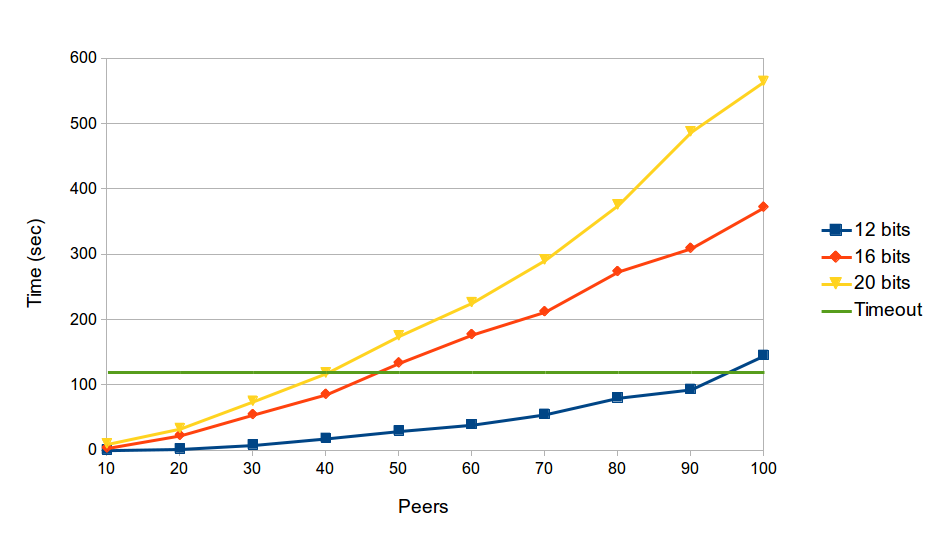
\includegraphics[width=\textwidth]{../Grapes/proof_of_work_graph.png}
\end{figure}

We see in Figure~\ref{graphs_pow} that with a proof of work requirement of 20 bits, it becomes infeasible to create much more than 40 peers, while more than 90 peers can effectively be created at 12 bits. In reality, one might wish to make the number of bits even higher.

It should be noted, that theoretically, the amount of time required should grow by 16 each time we increase the number of bits by 4. The reason our test shows nowhere near this huge increase is likely that the peers simply get more starved for connections, and form a much sparser network. This means that it is still possible to connect quite a few sybils to the network, but they will have a lesser effect on the other peers, due to their low connectivity.

\subsection{Finding optimal k-walker parameters}
\label{subsec:k_opti_params}
As described in section~\ref{subsec:base_system}, the k-walker algorithm implements an eventual delivery guarantee as long as the sender remains connected to the network by sending out walkers with exponentially increasing TTL at exponentially increasing intervals. Before doing the experiments comparing flooding and k-walkers we needed to find some optimal or at least pretty good parameters for this.

The required parameters were the starting values of wait time and TTL as well as how many walkers to send in parallel each time. Tested values of starting wait time include 0.5, 1, 2, 4, 8 and tested starting values of TTL include 8, 16, 32, 64, 128 and the tested numbers of walkers to send out time include 1, 2, 4, 8, 16, 32. Since each test took quite a while and had to be repeated several times to try different network layouts, we didn't test all possible combinations of the values but used our intuition and understanding of the effect of the values to zero in on some good values to test further. We found that the network layout had a huge effect on the time and number of passed messages in the network to send a single message and receive verification of delivery. We omit presenting the data from this experiments as not even close to every combination of the parameters were tested, making graphing the values useless, and not every test was written down. We ended up using a starting wait time of 4 seconds and starting TTL of 64 and send out 16 walkers in parallel.

\subsection{Flooding vs. k-walkers}
We tested the time and internal messages passed in the whole network by having two peers join a network of varying size and sending 10 messages from one to another, waiting for the acknowledgement of the previous message before sending the next. This test was then repeated to test various network layouts. These tests were performed with Proof-of-Work turned off and no artificial latency introduced in the system in network of size increments of 25 peers.

We weren't able to have networks involving more than 230 or so peers running on the same machine without random peers dying or at least not responding fast enough so we limit our testing to a max network size of 200.

\begin{figure}
\caption{K-Walker / Flooding: Time}
\label{graph_fvsk_t}
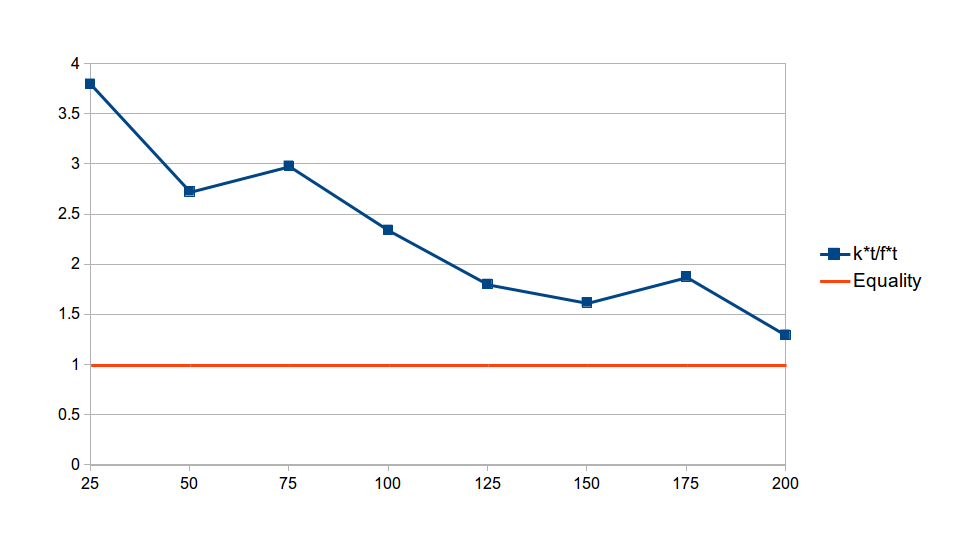
\includegraphics[width=\textwidth]{../Grapes/flooding_vs_kwalker_time_graph.png}
\end{figure}

\begin{figure}
\caption{K-Walker / Flooding: Messages}
\label{graph_fvsk_m}
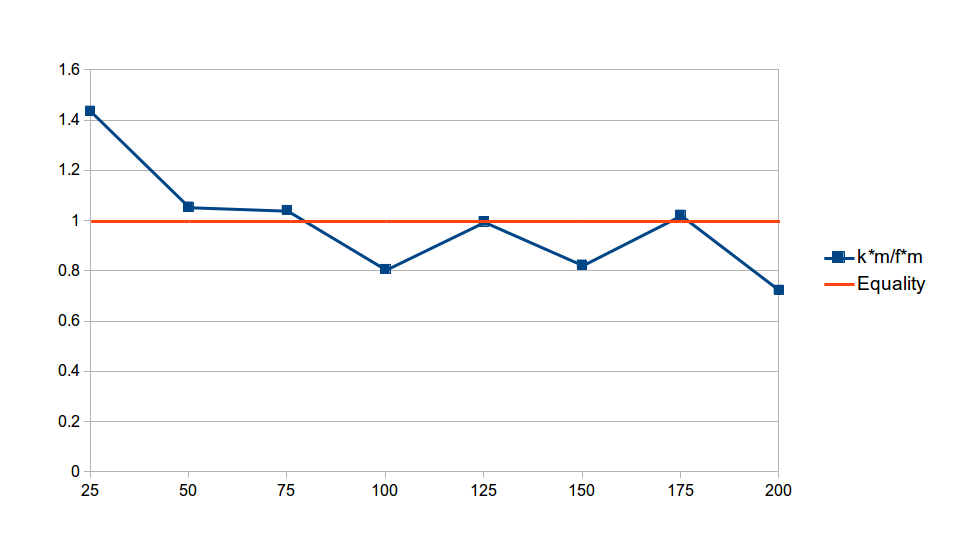
\includegraphics[width=\textwidth]{../Grapes/flooding_vs_kwalker_messages_graph.png}
\end{figure}

In Figure~\ref{graph_fvsk_t} we have graphed how the k-walker algorithm performs compared to flooding by dividing the time of the k-walker algorithm with time of the flooding algorithm run on the same network, then averaging this over 5 runs on different network of same size for a value in the final graph. The same was done for Figure~\ref{graph_fvsk_m}, except the number of messages for k-walkers and flooding was used instead.

We see in Figure~\ref{graph_fvsk_t} that kwalker in general takes more time than flooding, but also that its relative performance increases noticeably as network size grows. This suggests that the kwalker likely will outperform flooding in larger networks and, looking at the trendline, even in networks not much larger than our test sizes, perhaps at about 225 peers. In a realistic setting such as one of our use cases, we expect the network to reach much larger sizes, perhaps in the thousands, and so we expect a kwalker algorithm to perform much better than flooding time-wise in real world use.

In Figure~\ref{graph_fvsk_m} we see that the kwalker algorithm in general either outperforms or performs as well as flooding in regards to number of messages when ignoring very small network sizes.
If we had used different parameters for the kwalker algorithm, such as sending fewer walkers in parallel, we find it likely that kwalker would also have outperformed flooding at small network sizes. different parameters would also likely have been able to make the kwalker algorithm outperform flooding even more in larger networks
The graph seems to oscillate, only barely showing a trend towards better performance at larger networks. We explain this by the fact that the number of messages, as well as time, fluctuated greatly in our tests depending on the configuration of the exact network it was running on. It is also sad that we could not test on a network of a greater size than about 200 peers, as we expect the kwalker to be better at larger networks and we are unable to show it.

It should be noted that the kwalker algorithm waits a full 4 seconds after receiving no verification of delivery before sending out more walkers, and this will artificially inflate the time it takes on smaller networks where the wait time could easily be shorter as a verification walker will have a smaller network to traverse. Another disadvantage for the kwalker algorithm in this test, that also affects the amount of messages, is that it has a number of parameters which cannot be optimal for every network and network size, and we only spent a limited time trying to find some good parameters as can be seen in section~\ref{subsec:k_opti_params}.

\subsection{Cardinality of Diffie-Hellman Pools}

When working with the Pooled Diffie-Hellman connections, we wished to ensure that we made as few Diffie-Hellman negotions as possible. In order to measure this performance parameter, we started a network, and gave it time to settle down, while performing cover traffic. We then measured the average cardinality of the connection pools residing in the peers. This number should preferably be close to 1.

The test was done specifically with 100ms faked latency between peers, and by waiting 2 minutes while cover traffic and network kept generating data. We ran the test for 10 to 100 peers, in increments of 10. A higher number of peers was deemed unnecessary, as peers seemed to have little influence on the cardinality of the connection pools.

\begin{figure}
\caption{Cardinality}
\label{graph_cardinality}
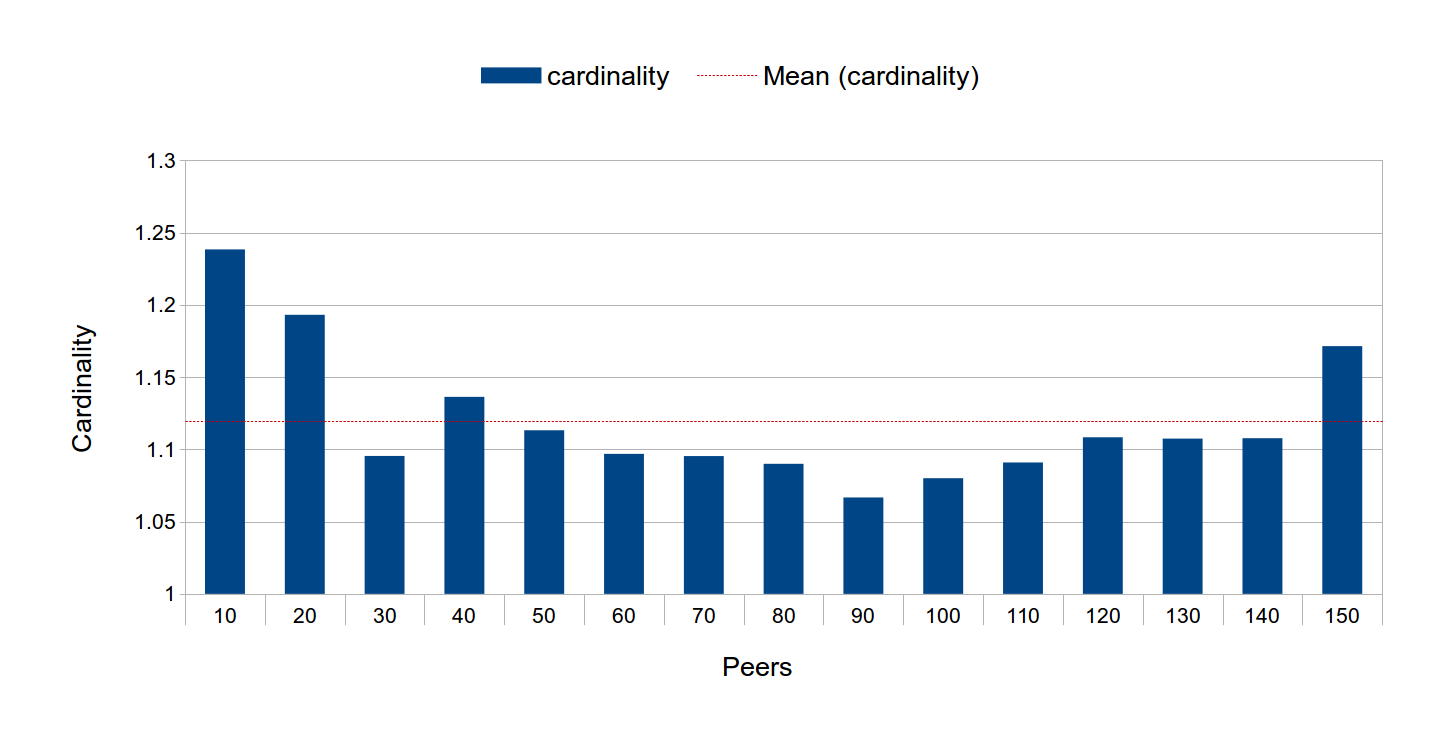
\includegraphics[width=\textwidth]{../Grapes/DH_pools_cardinality_graph.png}
\end{figure}

From this test, in Figure~\ref{graph_cardinality}, we see that we have a cardinality ranging between 1.07 and 1.25, which means that we are generating 7-25\% additional connections. The average amount of connection overshooting is very close to 12\% which we deem to be good. Note that the cardinality does not appear to rise with an increasing number of peers, and in fact the highest numbers seem to reside at very low peer numbers. We theorise that the high cardinality of low peer numbers might be caused by a greater amount of loops in the RPC call graph, leading to a forced additional connection.